% Chapter Template

\chapter{Introduction} % Main chapter title

\label{introduction} % Change X to a consecutive number; for referencing this chapter elsewhere, use \ref{ChapterX}

\lhead{\emph{Introduction}} % Change X to a consecutive number; this is for the header on each page - perhaps a shortened title

%----------------------------------------------------------------------------------------
%	SECTION 1
%----------------------------------------------------------------------------------------
\section{Introduction and motivation}

Lorem ipsum dolor sit amet, consectetur adipiscing elit. Aliquam ultricies lacinia euismod. Nam tempus risus in dolor rhoncus in interdum enim tincidunt. Donec vel nunc neque. In condimentum ullamcorper quam non consequat. Fusce sagittis tempor feugiat. Fusce magna erat, molestie eu convallis ut, tempus sed arcu. Quisque molestie, ante a tincidunt ullamcorper, sapien enim dignissim lacus, in semper nibh erat lobortis purus. Integer dapibus ligula ac risus convallis pellentesque.

Lorem ipsum dolor sit amet, consectetur adipiscing elit. Aliquam ultricies lacinia euismod. Nam tempus risus in dolor rhoncus in interdum enim tincidunt. Donec vel nunc neque. In condimentum ullamcorper quam non consequat. Fusce sagittis tempor feugiat. Fusce magna erat, molestie eu convallis ut, tempus sed arcu. Quisque molestie, ante a tincidunt ullamcorper, sapien enim dignissim lacus, in semper nibh erat lobortis purus. Integer dapibus ligula ac risus convallis pellentesque.

%-----------------------------------
%	SUBSECTION 1
%-----------------------------------
%\subsection{Subsection 1}
%
%Nunc posuere quam at lectus tristique eu ultrices augue venenatis. Vestibulum ante ipsum primis in faucibus orci luctus et ultrices posuere cubilia Curae; Aliquam erat volutpat. Vivamus sodales tortor eget quam adipiscing in vulputate ante ullamcorper. Sed eros ante, lacinia et sollicitudin et, aliquam sit amet augue. In hac habitasse platea dictumst.
%
%%-----------------------------------
%	SUBSECTION
%-----------------------------------
%\subsection{Subsection 2}
%
%Morbi rutrum odio eget arcu adipiscing sodales. Aenean et purus a est pulvinar pellentesque. Cras in elit neque, quis varius elit. Phasellus fringilla, nibh eu tempus venenatis, dolor elit posuere quam, quis adipiscing urna leo nec orci. Sed nec nulla auctor odio aliquet consequat. Ut nec nulla in ante ullamcorper aliquam at sed dolor. Phasellus fermentum magna in augue gravida cursus. Cras sed pretium lorem. Pellentesque eget ornare odio. Proin accumsan, massa viverra cursus pharetra, ipsum nisi lobortis velit, a malesuada dolor lorem eu neque.

%----------------------------------------------------------------------------------------
%	SECTION
%----------------------------------------------------------------------------------------
\section{Growth of air traffic movements in early 20th century}

Sed ullamcorper quam eu nisl interdum at interdum enim egestas. Aliquam placerat justo sed lectus lobortis ut porta nisl porttitor. Vestibulum mi dolor, lacinia molestie gravida at, tempus vitae ligula. Donec eget quam sapien, in viverra eros. Donec pellentesque justo a massa fringilla non vestibulum metus vestibulum. Vestibulum in orci quis felis tempor lacinia. Vivamus ornare ultrices facilisis. Ut hendrerit volutpat vulputate. Morbi condimentum venenatis augue, id porta ipsum vulputate in. Curabitur luctus tempus justo. Vestibulum risus lectus, adipiscing nec condimentum quis, condimentum nec nisl. Aliquam dictum sagittis velit sed iaculis. Morbi tristique augue sit amet nulla pulvinar id facilisis ligula mollis. Nam elit libero, tincidunt ut aliquam at, molestie in quam. Aenean rhoncus vehicula hendrerit.

%-----------------------------------
%	SUBSECTION
%-----------------------------------
\subsection{Years 2000 -- 2010}

First number to be shown is the total number of aircraft in the EU (fig. \ref{num_aircraft}). Trends for passenger aircraft and total number of aircraft show a slow in-crease of these numbers. Chain growth ratio of number of aircraft (fig. \ref{num_aircraft2}) shows a rapid increase in year 2006 and stabilization afterwards. At this point situation on European skies is rather comforting. But comparing these numbers with figure \ref{num_pass} may change the perspective.

\begin{figure}[h!]
\centering % bo \centering nie wstawia dodatkowego odstępu
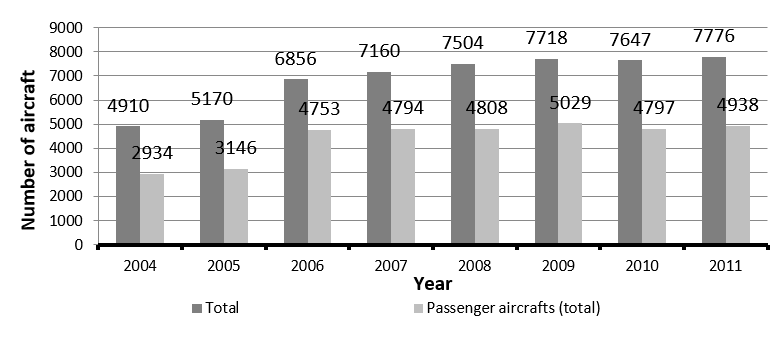
\includegraphics[width=0.85\textwidth]{Pictures/num_aircraft.png}
\caption{Number of aircraft registered in the EU (EUROSTAT)}
\label{num_aircraft}
\end{figure}

\begin{figure}[h!]
\centering % bo \centering nie wstawia dodatkowego odstępu
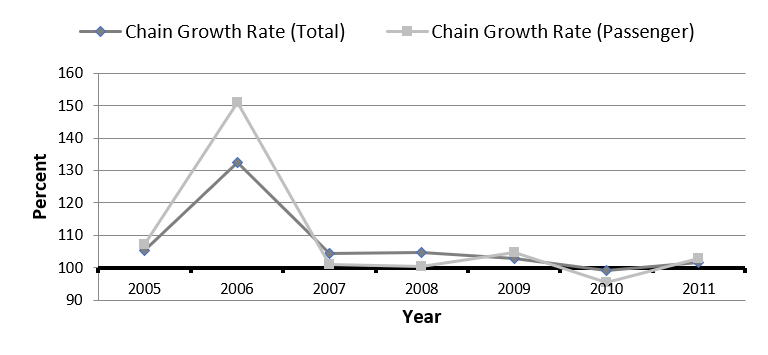
\includegraphics[width=0.85\textwidth]{Pictures/num_aircraft2.png}
\caption{Growth rate of number of aircraft registered in the EU}
\label{num_aircraft2}
\end{figure}

As by figure \ref{num_pass}, number of passengers is increasing, at average 50 to 70 million passengers every year. The growth rates (fig. \ref{num_pass2}) show large annual fluctuation of passenger count. Slowdown in year 2008 and decrease of passenger number in year 2009 are the aftermath of Financial Crisis of 2007-08. The situation recovers in years 2010-11. With roughly the same number of passenger airplanes (2007-11) this leads to rapid increase of passenger flights.

Existing fleet is supposed to deliver people and freight 24 hours a day, with very short overhaul periods, even shorter times to refuel and reload. Grounded aircraft generates loss instead of profit. Increasing number of flights generates yet another problem. All airplanes need an airfield with proper infrastructure to perform flight operations, basic maintenance, serve passengers and so on.

\begin{figure}[h!]
\centering % bo \centering nie wstawia dodatkowego odstępu
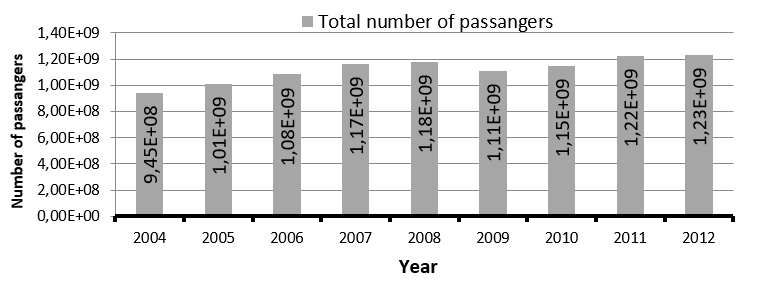
\includegraphics[width=0.85\textwidth]{Pictures/num_pass.png}
\caption{Total number of passengers in the EU (EUROSTAT)}
\label{num_pass}
\end{figure}

\begin{figure}[h!]
\centering % bo \centering nie wstawia dodatkowego odstępu
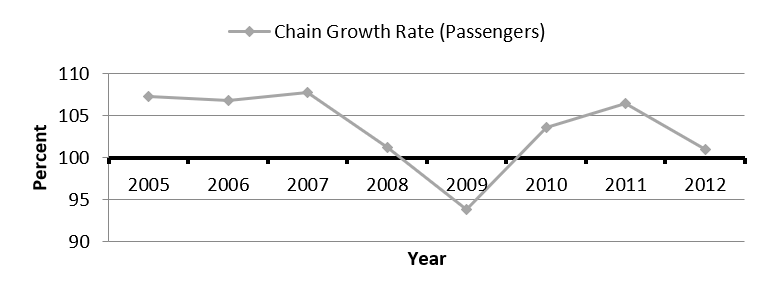
\includegraphics[width=0.85\textwidth]{Pictures/num_pass2.png}
\caption{Growth rate. Total number of passengers in the EU}
\label{num_pass2}
\end{figure}

Surprisingly, the number of main airports is not following the trend set up by number of passengers.  As seen on figure \ref{num_aerodrome} number of main airports (serving more than 150 000 passengers a year) remains roughly the same, with very slight increase in research period. Change in number of main airports (fig. \ref{num_aerodrome2}) is caused by varying number of passengers, rather than closing and opening airports. Decrease of number of airports in year 2009 is the aftermath of the economy crisis. Total number of airports varies among the years. This number includes small and medium airports such as club airfields and regional airports. Total number of airports (including registered regional and club airports) was under more influence of crisis and changed more rapidly.

\begin{figure}[h!]
\centering % bo \centering nie wstawia dodatkowego odstępu
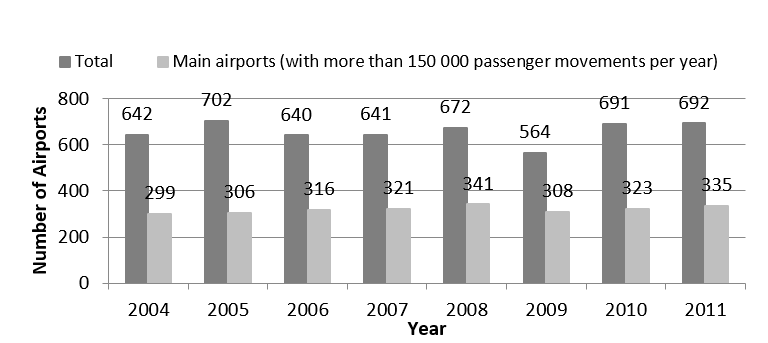
\includegraphics[width=0.85\textwidth]{Pictures/num_aerodrome.png}
\caption{Number of airports (EUROSTAT)}
\label{num_aerodrome}
\end{figure}

\begin{figure}[h!]
\centering % bo \centering nie wstawia dodatkowego odstępu
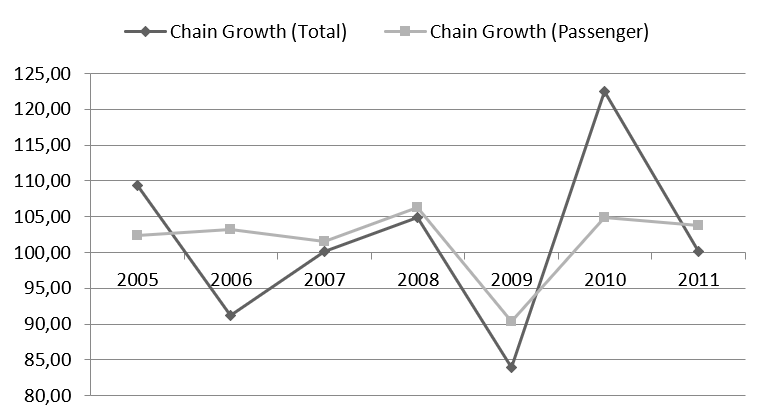
\includegraphics[width=0.85\textwidth]{Pictures/num_aerodrome2.png}
\caption{Growth rate. Number of airports (self study)}
\label{num_aerodrome2}
\end{figure}

%-----------------------------------
%	SUBSECTION
%-----------------------------------
\subsection{Years 2010 -- 2035}

Trends presented in previous section may not give the full perspective. Years 2001-2012 show a significant increase in air traffic in Europe. Expansion of the EU in year 2004, Financial Crisis of 2007-2008, Arab Spring trampling through the Middle East and Northern Africa all have their reflection in air movements on the continent. These factors make the predictions harder than simple extrapolation of data.

In order to show how air traffic will change, EUROCONTROL prepares medium and long term forecast for IFR movements. These forecasts are used mainly for planning purposes for airlines.

%Medium Term Forecast, prepared in September 2013 (latest available at editing this article) covers flight movements in EU airspace for years 2013-2019. Forecast is divided into short-term outlook for years 2013-2014 and long term – covering years up to 2019.
%
%As forecast states, after 2014, the traffic growth in Europe stabilizes at around 2.5\% increase per year showing rates higher in the 2015-2016 horizon (+2.7\%) than in the 2018-2019 horizon (2.4\%).
%
%Figures 7 and 8 show, that the growth is not uniform across Europe. While the growth in percentage terms is much weaker in the more mature markets of Western Europe, it is still the busiest States (Germany followed by France, Italy and UK) which will see the greatest number of extra flights per day be-tween now and 2019 (Fig. 2). Turkey will both be the fastest grower (5\% as average annual growth rate) and the biggest contributor of new flights to the European network in 2019 through both its domestic flights and international arrivals and departures.
%
%Medium term forecast takes into account limited capacity of airports. Air-port expansion is not taken into account in this prognosis, therefore figures presented are constrained.

Long term forecast, published in June 2013 covers IFR flight movements for years 2013-2035. Because of the range, the forecast is more robust and is divided into four scenarios \citep{growth_2013}

\begin{description}
\item[Scenario A: Global Growth (Technological Growth):] Strong economic growth in an increasingly globalized World, with technology used successfully to mitigate the effects of sustainability challenges such as the environment or resources availability.
\item[Scenario C: Regulated Growth:] Moderate economic growth, with regulation reconciling the environmental, social and economic demands to address the growing global sustainability concerns. This scenario has been constructed as the most likely of the four, most closely following the trends.
\item[Scenario C’: Happy Localism:] this scenario is introduced to investigate an alternative path for the future. With European economies being more and more fragile, increasing pressure on costs, stricter environmental constraints, air travel in Europe would adapt to new global environment but taking an inwards perspective. There would be less globalization, more trade inside EU (e.g. Turkey joining Europe is important in this scenario). Also, slow growth of leisure travel to outside Europe, however certainly more inside EU. More point-to-point traffic within Europe. It does not mean that Europe does not grow or does not adapt to new technologies and innovation but its main focus is local. Although this scenario is mostly based on scenario C (as its name indicates), it also inherits some aspects of other scenarios like higher fuel prices or low business aviation traffic of scenario D.
\item[Scenario D: Fragmenting World:] A World of increasing tensions between regions, with more security threats, higher fuel prices, reduced trade and transport integration and knock-on effects of weaker economies.
\end{description}

%\begin{figure}[h!]
%\centering % bo \centering nie wstawia dodatkowego odstępu
%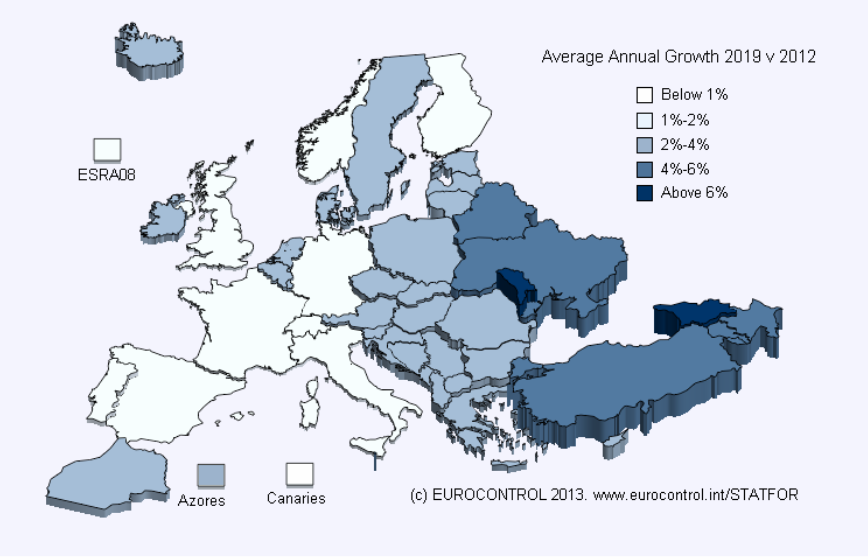
\includegraphics[width=0.85\textwidth]{Pictures/ec1.png}
%\caption{Average Annual Growth in IFR movements per State, 2019 vs. 2012 \citep{eurocontrol}}
%\label{ec1}
%\end{figure}
%
%\begin{figure}[h!]
%\centering % bo \centering nie wstawia dodatkowego odstępu
%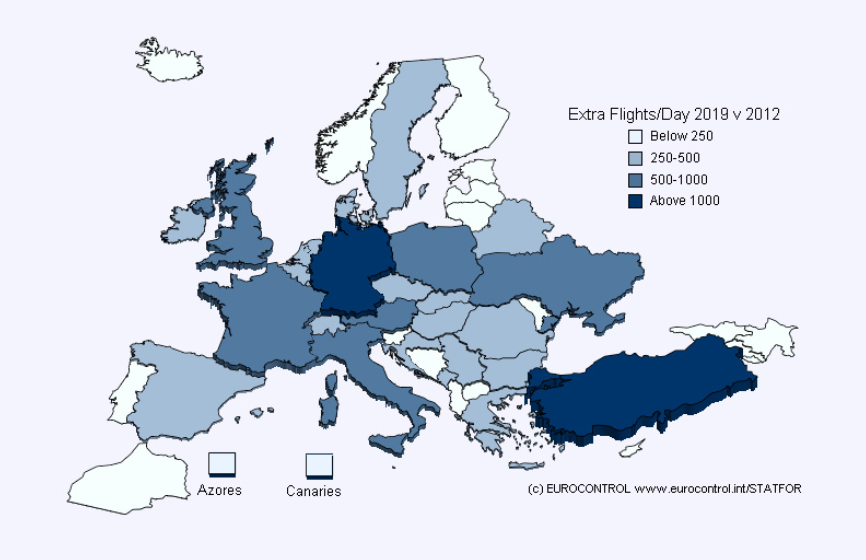
\includegraphics[width=0.85\textwidth]{Pictures/ec2.png}
%\caption{Number of additional movements per day for each state (2019 vs. 2012) \citep{eurocontrol}}
%\label{ec2}
%\end{figure}

Scenario C: Regulated growth is considered to be the most likely at point of publishing the report. This forecast predicts 14.4 million flights in Europe 2035, which is 1.5 times more than in 2012. That creates an average growth of 1.8\% per year. Forecast predicts that in 2025 traffic growth will decelerate due to predicted economic slowdown and reaching the capacity of airports.

As in medium term forecast, growth is not uniform across Europe. Due to lower starting point in calculations, more growth is expected in Eastern countries.

This however is not the full view on the situation. While growth will be faster in the East (figure \ref{scenarioC}), it is still mainly the big western countries that will need to deal with the greatest increase in the number of flights (figure \ref{totalflights}).

\begin{figure}[h!]
\centering % bo \centering nie wstawia dodatkowego odstępu
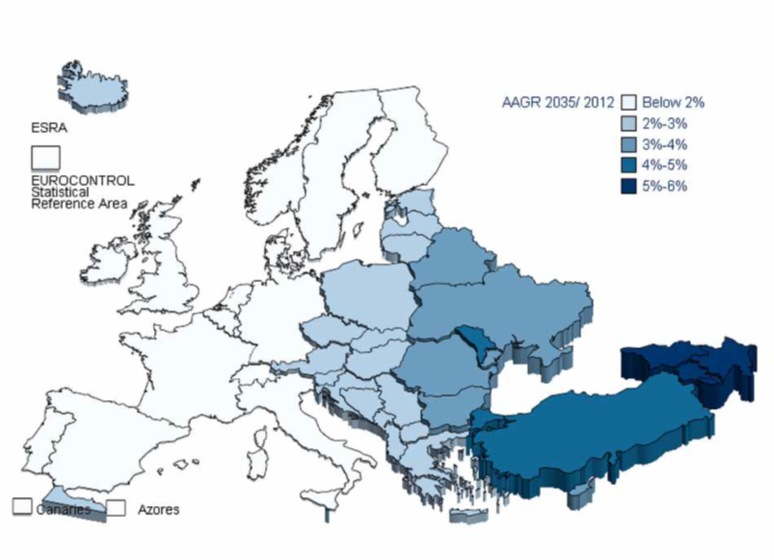
\includegraphics[width=0.85\textwidth]{Pictures/scenC.png}
\caption{Average annual growth (scenario C: Regulated Growth) \citep{eurocontrol}}
\label{scenarioC}
\end{figure}

\begin{figure}[h!]
\centering % bo \centering nie wstawia dodatkowego odstępu
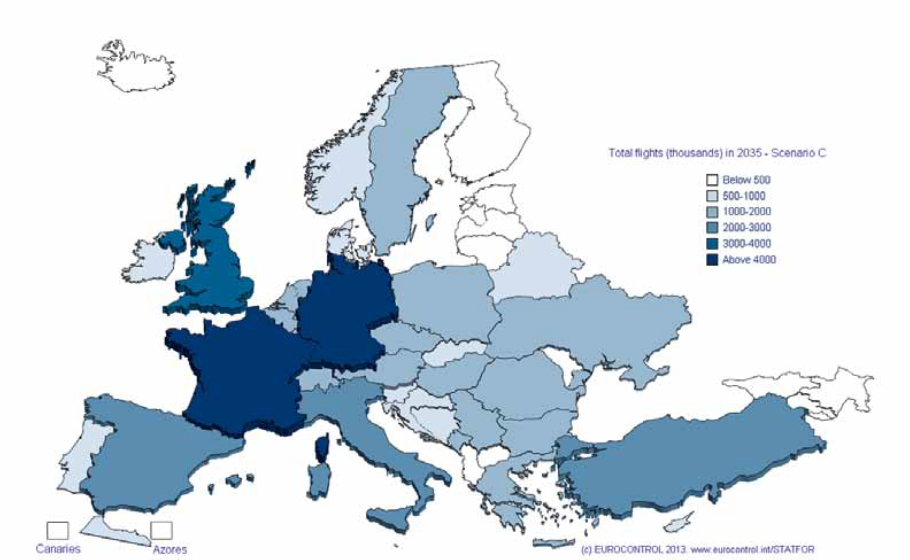
\includegraphics[width=0.85\textwidth]{Pictures/total2035.png}
\caption{Total traffic in 2035 \citep{eurocontrol}}
\label{totalflights}
\end{figure}

Presented forecasts show, that air traffic in Europe will grow significantly in the next few years. With no actions taken, two paths are available. On one hand, running such traffic on existing fleet with airports (reaching maximum capacity) located near city centers will create an environment filled with constant aircraft noise. On a preventive side, noise emission regulations are being tightened nearly every year. And the only way to conform strict regulations is to use state of the art engines and airplanes, because in this case, silence is golden.

%----------------------------------------------------------------------------------------
%	SECTION
%----------------------------------------------------------------------------------------
\section{Some excerpts from airworthiness regulations}

Sed ullamcorper quam eu nisl interdum at interdum enim egestas. Aliquam placerat justo sed lectus lobortis ut porta nisl porttitor. Vestibulum mi dolor, lacinia molestie gravida at, tempus vitae ligula. Donec eget quam sapien, in viverra eros. Donec pellentesque justo a massa fringilla non vestibulum metus vestibulum. Vestibulum in orci quis felis tempor lacinia. Vivamus ornare ultrices facilisis. Ut hendrerit volutpat vulputate. Morbi condimentum venenatis augue, id porta ipsum vulputate in. Curabitur luctus tempus justo. Vestibulum risus lectus, adipiscing nec condimentum quis, condimentum nec nisl. Aliquam dictum sagittis velit sed iaculis. Morbi tristique augue sit amet nulla pulvinar id facilisis ligula mollis. Nam elit libero, tincidunt ut aliquam at, molestie in quam. Aenean rhoncus vehicula hendrerit.

%-----------------------------------
%	SUBSECTION
%-----------------------------------
\subsection{CAEP regulations}

ICAO's current environmental activities are largely undertaken through the Committee on Aviation Environmental Protection (CAEP), which was established by the Council in 1983, superseding the Committee on Aircraft Noise (CAN) and the Committee on Aircraft Engine Emissions (CAEE).

The current structure of the Committee includes three working groups and four support groups. The working groups deal with the technical and operational aspects of noise reduction and mitigation, with the aircraft noise and emissions issues linked to airports and operations and with the technical and operational aspects of aircraft emissions. One support group provides information on the economic costs and environmental benefits of the noise and emissions options considered by CAEP, one addresses models and databases issues, one deals specifically with the ICAO Carbon Calculator and the last one is aimed at scientific understanding of aviation environmental impacts.
 
About once a year, CAEP meets as a Steering Group to review and provide guidance on the progress of the activities of the working groups. So far, CAEP has held eight formal meetings: in 1986 (CAEP/1), 1991 (CAEP/2), 1995 (CAEP/3), 1998 (CAEP/4,) 2001 (CAEP/5), 2004 (CAEP/6), 2007 (CAEP/7) and 2010 (CAEP/8). Each formal CAEP meeting produces a report with specific recommendations for the consideration of the ICAO Council. 

The Council acts on recommendations from CAEP in the light of any comments received from the Air Navigation Commission and, if there are economic aspects, from the Air Transport Committee. In the case of recommendations to introduce or amend Standards and Recommended Practices, there are established procedures for consulting States, after which the final decision rests with the Council.


%-----------------------------------
%	SUBSECTION
%-----------------------------------
\subsection{ICAO Annex 16}
Historically the oldest and presumably the most important regulations are stated in ICAO Annex 16 – Environmental Protection, Volume 1. First issue of this document was released in year 1981. At time of writing this article the latest issue is 6th, released in year 2011. Document contains standards (not strict requirements), Recommended Practices and Guide of the noise certification of aircraft that are operated in international air navigation, in accordance with the classification set out in the individual chapters: Each chapter describes different noise measurement points (Table \ref{annex16_1}) and noise levels for specific aircraft types:

\begin{enumerate}[a)]
\item Annex 16 Chapter 2 describes requirements for subsonic, jet engine propelled air-craft certified before 6th November 1977. With exceptions;
\item Annex 16 Chapter 3 describes requirements for:
\begin{itemize}
\item[-] Subsonic, jet engine propelled aircraft certified between 6th November 1977 and 1st January 2006,
\item[-] Propeller driven aircraft (MTOW over 8618 kg) certified between 1st January 1985 and 1st January 2006;
\end{itemize}
\item Annex 16 Chapter 4 describes requirements for:
\begin{itemize}
\item[-] Subsonic, jet engine propelled aircraft certified after 1st January 2006;
\item[-] Propeller driven aircraft (MTOW over 8618 kg) certified after 1st January 2006.
\end{itemize}
\end{enumerate}

Separate Chapters contain information on light aircraft (Annex 16 Chapter 7) and helicopters (Annex 16 Chapters 8 \& 11) and will not be discussed.

Table \ref{annex16_1} and \ref{annex16_2} contain a brief summarize of maximum noise levels and their measurement points. Noise levels and measurement points are not rigid. Maximum noise levels are logarithmic dependent from Maximum Take-Off Weight (MTOW) of certified aircraft. Highest noise levels are for heavier aircraft, with MTOW above 385 000 kg. Annex 16 fully describes weather requirements, flight procedures and equipment setup for proper measurements. Noise levels are presented in EPNdB (Effective Perceived Noise dB). This unit is not measurable in a direct manner. EPNdB calculations are based on measurements of noise level (measurements of acoustical pressure), spectrum of noise level and corrected with sustainability factors and noise damping of air (also dependent on weather). Methods on how to establish a measurement point, calculate correction factors from weather, wind, inaccurate measurement point are described in Annex or in its Addenda. Data presented below is an excerpt from chapters 2, 3 and 4 from 6th edition of ICAO Annex 16 (Table \ref{annex16_1}).

Maximum noise levels gained from Annex 16 are below 108 EPNdB. In comparison: Heavy traffic generates around 85dB, pneumatic road drill - circa 100dB, live rock concert generates circa 110-115dB noise. Exposition to noise level higher than 110dB for over 15 minutes may result in hearing damage. Short term (less than 10 minutes) exposure to 120 results in hearing damage, 130 dB is considered as a threshold of pain, 150dB causes eardrum rapture, while 194dB is considered as theoretical limit for sound barrier at 1 atmosphere of pressure.

Noise levels appear to be high. But such levels occur only in the nearest vicinity of the airport. Concerning that nearly any main airport in Europe is surrounded by a large perimeter, nearest housing areas are subjected to noise levels that are safe, but may be considered as annoying. Also, many airports create their own noise requirements and do not allow air traffic operations of aircraft not conforming to such.

\begin{table}[]
\centering
\caption{Noise measurement points per ICAO Annex 16 \citep{annex16}}
\label{annex16_1}
\resizebox{\textwidth}{!}{%
\begin{tabular}{l|lll} \toprule
\multicolumn{1}{c}{\multirow{2}{*}{Chapter}} & \multicolumn{3}{l}{Noise measurement point} \\
\multicolumn{1}{c}{} & Name & Distance & Point \\ \midrule
\multirow{3}{*}{2} & Sideway & 650m & On line parallel to runway where measured noise is max \\
 & Fly-by & 6.5km & On extent of runway axis measured from start of take-off \\
 & Approach & 2000m & From runway threshold below approach path \\ \midrule
\multirow{4}{*}{3, 4} & Sideway (jet) & 450m & On line parallel to runway where measured noise is max \\
 & Sideway (prop) & 650m & Below take-off path for take-off power climb \\
 & Fly-by & 6.5km & On extent of runway axis measured from start of take-off \\
 & Approach & 2000m & From runway threshold below approach path \\ 
\bottomrule
\end{tabular}%
}
\end{table}

\begin{table}[]
\centering
\caption{Maximum noise levels per ICAO Annex 16 \citep{annex16}}
\label{annex16_2}
\begin{tabular}{l|lrr} \toprule
\multicolumn{1}{c}{Chapter} & \multicolumn{1}{c}{Point} & \multicolumn{1}{c}{Engine count} & \multicolumn{1}{c}{Maximum EPNdB} \\ \midrule
\multirow{3}{*}{2} & Sideway & N/A & 108-102 \\
 & Fly-by & N/A & 108-93 \\
 & Approach & N/A & 108-102 \\ \midrule
\multirow{5}{*}{3, 4} & Sideway & N/A & 103-94 \\
 & \multirow{3}{*}{Fly-by} & 1 or 2 & 101-89 \\
 &  & 3 & 104-89 \\
 &  & 4 & 106-89 \\
 & Approach & N/A & 105-98 \\
\bottomrule
\end{tabular}
\end{table}


%-----------------------------------
%	SUBSECTION
%-----------------------------------
\subsection{Local regulations}

One of the airports with most strict noise requirements is London Heathrow. It is the third busiest airport in the world, serving more than 70 million passengers in 2012 and handling more international passengers than any other airport in the world.

In order to prevent nearby housing areas from noise effects, particularly at night, Heathrow airport introduced their own regulations for incoming and departing traffic. Air traffic Control at Heathrow Approach Control guides traffic incoming from four major routes into one approach stream. When possible, Controllers advise the use of Continuous Descent Approach (CDA). CDA allows for a smooth, constant-angle descent to landing (Fig. \ref{cda}). A continuous descent approach starts ideally from the top of descent, i.e. at cruise altitude, and allows the aircraft flying its individual optimal vertical profile down to runway threshold.

\begin{figure}[h!]
\centering % bo \centering nie wstawia dodatkowego odstępu
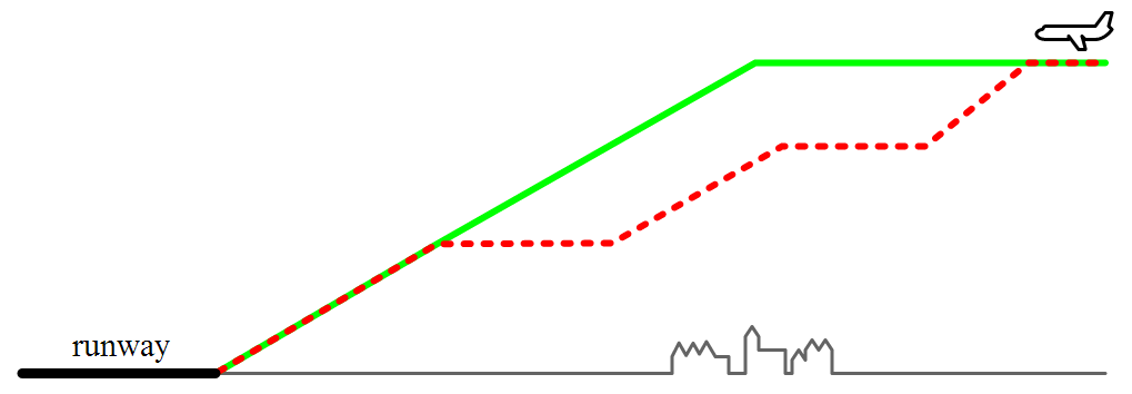
\includegraphics[width=0.85\textwidth]{Pictures/cda.png}
\caption{CDA approach (solid line) vs. Standard approach (dash line)}
\label{cda}
\end{figure}

Night-time flights at Heathrow are subject to restrictions. Between 23:00 and 07:00, the noisiest aircraft (rated QC/8 and QC/16) cannot be scheduled for operation. In addition, during the night quota period (23:30–06:00) there are four limits:

\begin{itemize}
\item[-] A limit on the number of flights allowed;
\item[-] A quota count system which limits the total amount of noise permitted, but allows operators to choose to operate fewer noisy aircraft or a greater number of quieter planes;
\item[-] QC/4 aircraft cannot be scheduled for operation;
\item[-] A voluntary agreement with the airlines that no early morning arrivals will be scheduled to land before 04:30.
\end{itemize}

A trial of "noise relief zones" ran from December 2012 to March 2013, which concentrated approach flight paths into defined areas compared with the existing paths which were spread out. The zones used alternated weekly, meaning residents in the "no-fly" areas received respite from aircraft noise for set periods. However, it was concluded that some residents in other areas experienced a significant dis-benefit as a result of the trial and that it should therefore not be taken forward in its current form.

The Quota Count (QC) system was introduced on Heathrow in 1993. Each aircraft is classified and awarded a grade, called a Quota Count, based on how much noise it generates. Quieter aircraft are given a smaller grade.  Aircraft are classified separately for landing and take-off. Take-off quota count values are based on the average of the certificated flyover and sideline noise levels at maximum take-off weight, with 1.75 EPNdB added for ICAO Annex 16 Chapter 2 aircraft. Landing quota count values are based on the certificated approach noise level at maximum landing weight minus 9.0 EPNdB.

Noise classification for aircraft is described in Table \ref{tab:qc1}. Examples of aircraft classified in the QC system are presented in Table \ref{tab:qc2}.

Noise levels required by Heathrow Airport are far stricter than those stated in ICAO Annex 16. Such restrictions result in relatively noise friendly environment around Heathrow. ERCD report 1101 – Noise Exposure Contours for Heathrow Airport \citep{ERCD}, prepared by Environmental Research and Consultancy Department of British Civil Aviation Authority shows the effect of Heathrow Airport traffic on nearby locations. Report prepared in year 2010, presents number and location of households affected by specific noise levels generated by Heathrow air traffic (Fig. \ref{heathrow}).

\begin{figure}[h!]
\centering % bo \centering nie wstawia dodatkowego odstępu
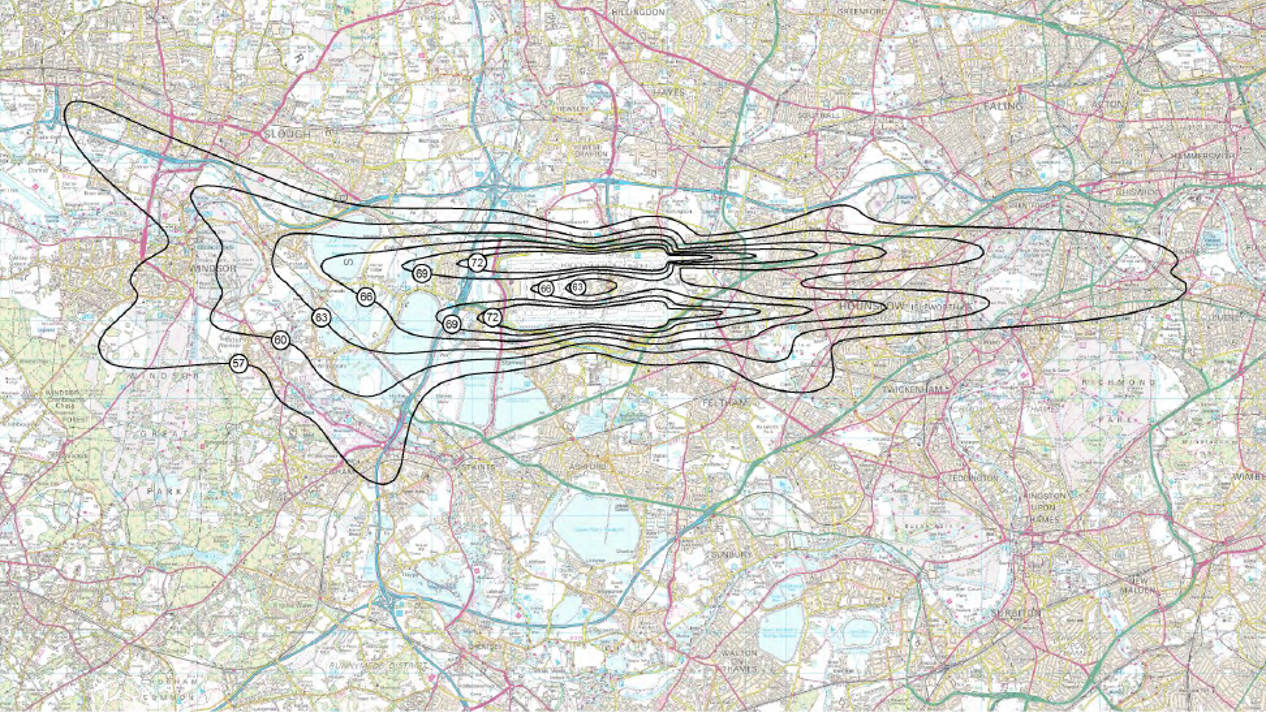
\includegraphics[width=0.85\textwidth]{Pictures/heathrow.png}
\caption{Heathrow air traffic noise contours. 83\% western and 17\% eastern traffic \citep{ERCD}}
\label{heathrow}
\end{figure}

Noise contours (Fig. \ref{heathrow}) show that 83dB of perceived noise level contains the terminal area, 72dB -- in the nearest vicinity of the runway and 66dB outside the aerodrome premises. 60dB noise is comparable to normal office space or restaurant rustle. 70dB is the sound level of moderate traffic and may be annoying to some people.

\begin{table}[]
\centering
\caption{Noise Quota Count classification in Heathrow \citep{ERCD}}
\label{tab:qc1}
\begin{tabular}{@{}rl@{}}
\toprule
Noise Classification & Quota Count \\ \midrule
Below 84 EPNdB & Exempt \\
84-86.9 EPNdB & 0.25 \\
87-89.9 EPNdB & 0.5 \\
90-92.9 EPNdB & 1 \\
93-95.9 EPNdB & 2 \\
96-98.9 EPNdB & 4 \\
99-101.9 EPNdB & 8 \\
Greater than 101.9 EPNdB & 16 \\ \bottomrule
\end{tabular}
\end{table}

\begin{table}[]
\centering
\caption{Examples of QC aircraft classification \citep{ERCD}}
\label{tab:qc2}
\begin{tabular}{@{}rll@{}}
\toprule
Aircraft type & QA Departure & QC Arrival \\ \midrule
Airbus A320 family & 0.5-1 & 0.25-0.5 \\
Airbus A380 & 2 & 0.5 \\
Boeing 737 Classic & 0.25-0.5 & 1 \\
Boeing 747-400 & 4 & 2 \\
Boeing 747-8 & 2 & 1 \\
Boeing 757-200 & 0.5 & 0.25 \\
Boeing 767-300 & 1 - 2 & 1 \\
Boeing 777-200ER & 2 & 1 \\
Embraer 145 & 0.25 & 0.25 \\ \bottomrule
\end{tabular}
\end{table}

This concludes that Heathrow airport restricts the movements of really loud airships to prevent its neighbors from aircraft noise. Presumably, Heathrow restrictions will lower the acceptable noise levels even more, due to increasing air traffic and urban sprawl around the airport.

%----------------------------------------------------------------------------------------
%	SECTION
%----------------------------------------------------------------------------------------
\section{Influence of regulations on engineering solutions}

Sed ullamcorper quam eu nisl interdum at interdum enim egestas. Aliquam placerat justo sed lectus lobortis ut porta nisl porttitor. Vestibulum mi dolor, lacinia molestie gravida at, tempus vitae ligula. Donec eget quam sapien, in viverra eros. Donec pellentesque justo a massa fringilla non vestibulum metus vestibulum. Vestibulum in orci quis felis tempor lacinia. Vivamus ornare ultrices facilisis. Ut hendrerit volutpat vulputate. Morbi condimentum venenatis augue, id porta ipsum vulputate in. Curabitur luctus tempus justo. Vestibulum risus lectus, adipiscing nec condimentum quis, condimentum nec nisl. Aliquam dictum sagittis velit sed iaculis. Morbi tristique augue sit amet nulla pulvinar id facilisis ligula mollis. Nam elit libero, tincidunt ut aliquam at, molestie in quam. Aenean rhoncus vehicula hendrerit.